


\documentclass[12pt,a4paper]{article}


%Spacing Packages
\usepackage{fullpage}
\usepackage{a4wide}

%Other Packages
\usepackage{amssymb}
\usepackage{amsmath}
\usepackage{euscript}
\usepackage{graphicx}
\usepackage{enumerate}

\usepackage[lf]{venturis} %% lf option gives lining figures as default; 
			  %% remove option to get oldstyle figures as default
\usepackage[T1]{fontenc}


\begin{document}

\begin{quote}

\begin{center} {\large 24.118 -- Paradox and Infinity \\ \vspace{1mm}}
 {\large Problem Set 7: Non-Measurable Sets \\ \vspace{1mm}}
 
\end{center}
\vspace{3mm}

\noindent How these problems will be graded:

\begin{itemize} 

\item For questions 1, 2 and 3a and 3b, you will be graded both on the basis of whether your answers are correct and on the basis of whether they are properly justified. There is no word limit for those questions.

\item For questions 3c and 4, you will be graded on the basis of the \emph{reasons} you give in support of your answer, rather than the answer itself. But you must give your
answer to each in less than 250 words.

\end{itemize} 

\end{quote} 


\subsection*{Problems:}


\begin{enumerate}

\item  Consider an infinite sequence of coin tosses, one for each natural number $0, 1, 2,\ldots$ Each time the coin lands Heads we write down a ``0'', and each time it lands Tails
we write down a ``1''. The result is an infinite sequence of zeroes and ones, which corresponds to an element of $[0, 1]$; specifically: the number whose binary representation is ``0.'' followed by the sequence of zeroes and ones we got from our coin tosses.

For some natural number $k$, let $m$ and $n$ be integers such that $0 \le m < n \le 2^k$. Show that if the coin is fair, then the probability of picking a number in the interval $[\frac{m}{2^k}, \frac{n}{2^k}]$ is $\frac{n-m}{2^k}$. (3 points)
	
\item Consider the \textbf{Cantor Set} (named for our old friend Georg Cantor, but actually first described by Irish mathematician Henry John Stephen Smith, and discovered independently by several others). You get the Cantor set by 
\begin{itemize}
\item Stage 0: starting with the interval $[0,1]$, 
\item Stage 1: removing the middle third open interval $(\frac{1}{3},\frac{2}{3})$; 
\item Stage 2: then removing the middle third open intervals of the remaining bits: $(\frac{1}{9}, \frac{2}{9})$  and $(\frac{7}{9},\frac{8}{9})$;
\item Stage 3: then again removing the middle third open intervals of what remains; 
\item And so on\ldots
\end{itemize}

There is a stage for every natural number. The Cantor Set is what is left over after all the stages.

Here is a picture of the first seven steps in the process:

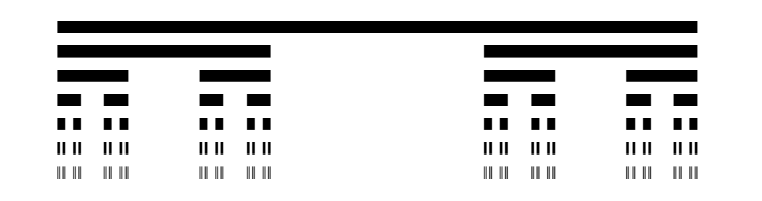
\includegraphics[scale=0.5]{755px-Cantor.png}

\begin{enumerate}
\item What is the Lebesgue measure of the what gets taken away during Stage 1? What about what gets taken away during Stage 2? What about Stage 3? What about Stage $n$? (3 points)
\item What is the Lebesgue measure of what is gone after all stages are done? (2 points)
\item What is the Lebesgue measure of the Cantor set? (2 points)
\end{enumerate}

\item Let $S$ be the set of all functions from natural numbers to $\{0,1\}$.  For $f_1, f_2 \in S$, say that $f_1$ is in the same ``orbit'' as $f_2$ iff there are at most finitely many numbers $k$ such that $f_1(k) \neq f_2(k)$.
\begin{enumerate}

\item Show that ``being in the same orbit'' is an equivalence relation. (In other words, show that if $f_1,f_2, f_3\in S$, then (i) $f_1$ is in the same orbit as itself, (ii) if $f_1$ is
in the same orbit as $f_2$, then $f_2$ is in the same orbit as $f_1$, and (iii) if $f_1$ is in the same orbit as $f_2$ and $f_2$ is in the same orbit as $f_3$, then $f_1$ is in the same
orbit as $f_3$.) (1 points)

\item Let $f_0(n) = 0$ for every $n$, and let $O_0$ be $f_0$'s orbit. Describe a function $g_0$ that assigns each member of $O_0$ to a different natural number. (3 points)

\item Given an arbitrary orbit $O$, is it possible to describe a function that assigns each member of $O$ to a different natural number? If so, describe one such function;
if not, explain why not. (3 points)

\end{enumerate}

\item The Banach-Tarski Theorem shows that at least one of the four following propositions is true:
\begin{enumerate}[(i)]
\item It is possible for the volume of a set to change when it is rotated (i.e., the correct measure for volume is not uniform).
\item It is possible for the volume of the union of two disjoint sets to be different from the sum of their volumes (i.e., we should not be using a finitely additive measure for volume).
\item Not all sets of points in a three-dimensional space have a volume (i.e., the standard solution).
\item The Axiom of Choice is false.
\end{enumerate}

If you have to accept one of these, which do you accept? Why? (6 points)

\end{enumerate}

\end{document}





